% !TEX program = pdflatex
% HC 6001 -- Dr. Castillo -- lecture of 2024-11-14 / 2024-11-19
% Transcription of the 7-page manuscript "SMALL OSCILLATIONS (Chapter 6 Goldstein)".
%
% Per-lecture symbol declarations live in this preamble, per SYMBOL_CONVENTIONS.md:
%   eta, eta_j            small displacement, q_j = q_{0j} + eta_j
%   eta_{j0}, delta_j     normal-mode amplitude and phase
%   T_ij, V_ij            kinetic / potential matrices (components, plain letters)
%   V, T, A, 1            the same objects AS MATRICES, in the doubled letterform
%   zeta, zeta_k          normal coordinates
%   l                     A LENGTH (mgl, omega_0^2 = g/l) -- never angular momentum
%   k                     mode index k = 1..n (the "SIMPLE CASE" panel on p. 2 is the
%                         lecturer's own local reuse of k as a spring constant)
%   nu                    initial angular speed, phidot_1 = -phidot_2 = nu > 0
%   x                     = omega_0^2 / omega^2 (p. 5)

\documentclass[11pt]{article}
\usepackage{goldsteinnotes}
\usepackage{xcolor}
\usepackage{bbm}
\usepackage{float}

% --- the doubled letterforms the lecturer uses for matrices -------------------
% T is BOTH the kinetic energy and the mass matrix on the same page; losing the
% distinction breaks 1 = A^dagger T A and [V - omega_k^2 T] a_k = 0.
\newcommand{\Vm}{\mathbb{V}}
\newcommand{\Tm}{\mathbb{T}}
\newcommand{\Am}{\mathbb{A}}
\newcommand{\Idm}{\mathbbm{1}}

% --- struck-out material inside mathematics ---------------------------------
\newcommand{\rmath}[1]{\text{\retracted{\ensuremath{#1}}}}

% --- the lecturer's pen colours, which carry meaning on pp. 1 and 4 ----------
\definecolor{notesred}{rgb}{0.85,0.05,0.05}
\definecolor{notesblue}{rgb}{0.15,0.15,0.85}
\definecolor{notesgreen}{rgb}{0.00,0.55,0.15}
\definecolor{typedink}{rgb}{0.30,0.30,0.34}

% --- typed (non-manuscript) annotations on p. 7 ------------------------------
\newcommand{\typednote}[1]{%
  \par\vspace{5pt}%
  \noindent
  {\color{typedink}\rule{2pt}{2.4\baselineskip}}\hspace{6pt}%
  \begin{minipage}[b]{\dimexpr\linewidth-18pt}
    {\sffamily\scriptsize\color{typedink}
      [typed annotation on the manuscript page --- not in the lecturer's hand]}\\
    {\sffamily\small\color{typedink} #1}
  \end{minipage}%
  \par\vspace{5pt}}

\newcommand{\tnote}[1]{\footnote{\emph{Transcriber's note.} #1}}

% --- Dirac notation, used only in the closing QM comparison ------------------
\providecommand{\ket}[1]{\left|#1\right\rangle}
\providecommand{\braket}[2]{\left\langle #1 \middle| #2 \right\rangle}

\title{\textbf{Small Oscillations}\\[2pt] \large (Chapter 6 Goldstein)}
\author{HC 6001 \quad--\quad Dr.\ Castillo}
\date{14 and 19 November 2024}

\begin{document}
\maketitle

\section*{1D case}

\begin{equation*}
  \ddot q = f(q),
  \qquad
  \text{EQUILIBRIUM at } q = q_0
  \iff
  0 = f(q_0).
\end{equation*}

Now we want to know what happens if we move a little bit away from $q_0$:
\begin{equation*}
  q = q_0 + \eta,
  \qquad \eta \ \text{``SMALL''}.
\end{equation*}
\begin{equation*}
  (q_0+\eta)^{\bm{\cdot\cdot}} = \ddot\eta,
  \qquad\qquad
  f(q_0+\eta) = \overset{0}{\rmath{f(q_0)}} + \eta\, f'(q_0) + \cdots
\end{equation*}
\begin{equation*}
  \ddot\eta \simeq f'(q_0)\,\eta
  \qquad \text{SMALL DEVIATION}
\end{equation*}
\begin{center}
  (EQUATION OF MOTION IS \textcolor{notesred}{LINEAR} IN SMALL DEVIATIONS)
\end{center}

\begin{align*}
  \text{OSCILLATIONS} &\iff f'(q_0) < 0,
    & \omega &= \sqrt{-f'(q_0)},
    & \eta &= \eta_0 \cos(\omega t + \varphi_0),\\
  \text{INSTABILITY}  &\iff f'(q_0) > 0,
    & \lambda &= \sqrt{f'(q_0)},
    & \eta &= A e^{\lambda t} + B e^{-\lambda t}.
\end{align*}

\hrule\vspace{6pt}

\section*{More than one degree of freedom}

(Simplify by assuming $V = V(q_1 \cdots q_n, t)$.)
\begin{equation*}
  L = T - V
\end{equation*}
\begin{gather*}
  \left.\text{Equilibrium at } (q_1 \cdots q_n) = (q_{01}\cdots q_{0n}) \right\}
  \iff
  \text{GENERALIZED FORCES}\\[2pt]
  Q_j = -\evalat{\pd{V}{q_j}}{\vec q = \vec q_0} = 0 .
\end{gather*}

\begin{figure}[htbp]
  \centering
  \begin{minipage}[b]{0.50\textwidth}
    \centering
    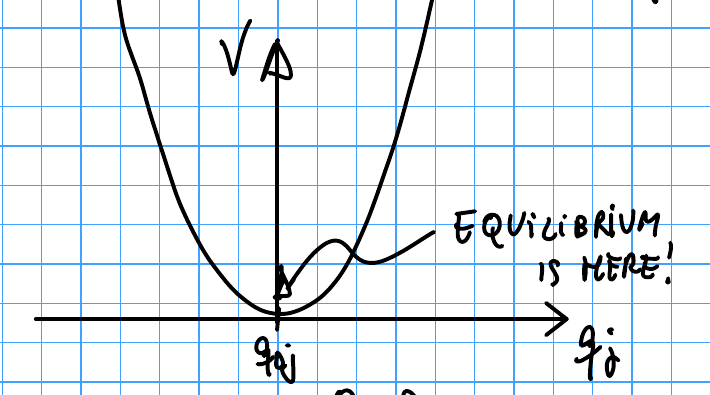
\includegraphics[width=\linewidth]{figures/fig_pe_equilibrium.png}
  \end{minipage}\hfill
  \begin{minipage}[b]{0.44\textwidth}
    \centering
    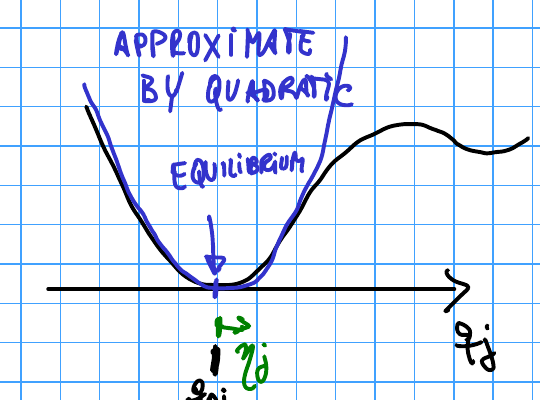
\includegraphics[width=\linewidth]{figures/fig_pe_quadratic.png}
  \end{minipage}
  \caption{Left: the potential $V$ against $q_j$; the minimum at $q_{0j}$ is
  marked ``EQUILIBRIUM IS HERE!''. Right: the same well with the
  \textcolor{notesblue}{blue} ``APPROXIMATE BY QUADRATIC'' curve laid over it, the
  \textcolor{notesblue}{blue} arrow labelling the equilibrium point, and the
  \textcolor{notesgreen}{green} displacement $\eta_j$ measured from $q_{0j}$ ---
  the only place in the lecture where the small-displacement variable is
  introduced graphically.}
\end{figure}

\subsection*{Taylor expand $V$ to 2nd order in $\eta$}

\begin{align*}
  V(q_1 \cdots q_n)
  &= \underbrace{V(q_{01}\cdots q_{0n})}_{\substack{\text{CONSTANT}\\ \Rightarrow\ \text{NO WORRIES}}}
   + \sum_{j=1}^{n}
     \underbrace{\rmath{\evalat{\pd{V}{q_j}}{\vec q_0}}}_{\substack{-Q_j = 0\\[2pt] 0}}\eta_j
   + \frac{1}{2}\sum_{i,j=1}^{n}
     \underbrace{\evalat{\frac{\partial^2 V}{\partial q_i\,\partial q_j}}{\vec q_0}}_{\equiv\, V_{ij}}
     \eta_i\eta_j
   + \rmath{O(\eta^3)} ,\\[4pt]
  & \qquad q_j = q_{0j} + \eta ,
  \qquad V_{ij} \ \text{an } n\times n \text{ MATRIX},
  \qquad V_{ij} = V_{ji}.
\end{align*}

\begin{equation*}
  T = \frac{1}{2}\sum_{i,j=1}^{n}
      \underbrace{\evalat{\frac{\partial^2 T}{\partial \dot q_i\,\partial \dot q_j}}
                        {\substack{\dot{\vec q}=0\\ \vec q = \vec q_0}}}_{T_{ij}}
      \dot\eta_i\dot\eta_j ,
  \qquad
  T_{ij} = T_{ji} .
\end{equation*}

\begin{equation*}
  \boxeq{\;
  \begin{aligned}
    T &= \sum_{p=1}^{N} \frac{m_p}{2}\bigl(\dot{\vec r}_p\bigr)^2 \\[2pt]
    \dot{\vec r}_p &= \sum_{j=1}^{n} \pd{\vec r_p}{q_j}\,\dot q_j
      + \rmath{\pd{\vec r_p}{t}}
      \qquad \text{\small(ASSUME)}
  \end{aligned}\;}
\end{equation*}

\section*{Lagrangian, Lagrange equations and the eigenvalue problem}

\begin{equation*}
  \boxeq{\;
    L = \frac{1}{2}\sum_{i,j=1}^{n}
        \bigl( T_{ij}\,\dot\eta_i\dot\eta_j - V_{ij}\,\eta_i\eta_j \bigr) \;}
\end{equation*}

\begin{align*}
  \pd{}{\eta_2}\!\left(\frac{1}{2}\bigl[
      V_{11}\eta_1\eta_1 + V_{12}\eta_1\eta_2 + V_{21}\eta_2\eta_1 + V_{22}\eta_2\eta_2
    \bigr]\right)
  &= \frac{1}{2}\bigl[(V_{12}+V_{21})\eta_1 + 2V_{22}\eta_2\bigr]
   = V_{21}\eta_1 + V_{22}\eta_2 ,
\end{align*}
using $V_{12} = V_{21}$.
\begin{center}
  ($\tfrac{1}{2}$ PREFACTOR CANCELS WITH FACTOR OF 2 IN THE DERIVATIVE)
\end{center}

In general:
\begin{equation*}
  \pd{L}{\eta_i} = -\sum_{j=1}^{n} V_{ij}\,\eta_j ,
  \qquad\qquad
  p_i = \pd{L}{\dot\eta_i} = \sum_{j=1}^{n} T_{ij}\,\dot\eta_j .
\end{equation*}

Lagrange Eqns:
\begin{equation*}
  0 = \pd{L}{\eta_i} - \dot p_i
  \qquad\Longrightarrow\qquad
  \boxeq{\;0 = \sum_{j=1}^{n} -V_{ij}\,\eta_j - \sum_{j=1}^{n} T_{ij}\,\ddot\eta_j\;}
  \qquad i = 1,\dots,n .
\end{equation*}

\begin{center}
\fbox{\begin{minipage}{0.86\textwidth}
\textsc{Simple case.}
\begin{gather*}
  T = \frac{m}{2}\dot\eta^2 , \qquad V = \frac{k}{2}\eta^2 ,
  \qquad L = \frac{m}{2}\dot\eta^2 - \frac{k}{2}\eta^2 ,\\
  \pd{L}{\eta} = -k\eta , \qquad \pd{L}{\dot\eta} = m\dot\eta ,\\
  0 = \pd{L}{\eta} - \ddt{}\!\left(\pd{L}{\dot\eta}\right) = -k\eta - m\ddot\eta
  \qquad\Longrightarrow\qquad
  \boxeq{\;m\ddot\eta = -k\eta\;}
\end{gather*}
\end{minipage}}
\end{center}

Propose:
\begin{equation*}
  \eta_j = \eta_{j0}\cos(\omega t + \delta_j)
  \quad\Longrightarrow\quad
  \ddot\eta_j = -\omega^2 \eta_j ,
  \qquad i = 1,\dots,n .
\end{equation*}
\begin{equation*}
  0 = \sum_{j=1}^{n}\bigl(V_{ij}\eta_j - \omega^2 T_{ij}\eta_j\bigr)
    = \sum_{j=1}^{n}\bigl(V_{ij} - \omega^2 T_{ij}\bigr)\eta_{j0}\cos(\omega t + \delta_j) ,
  \qquad i = 1,\dots,n .
\end{equation*}

BUT ALSO, since $\cos(\omega t + \delta_j)\neq 0$ for most times:
\begin{equation*}
  \boxeq{\;
    0 = \sum_{j=1}^{n}
        \bigl(\underset{\text{EIGENVALUE}}{V_{ij} - \omega^2 T_{ij}}\bigr)\,
        \underset{\text{EIGENVECTOR}}{\eta_{j0}} \;}
  \qquad i = 1,\dots,n
\end{equation*}
\begin{center}
  $\omega$: NORMAL MODE FREQUENCY \qquad $\eta_{j0}$: NORMAL MODE
\end{center}

For the $\eta_{j0}$ to be nontrivial, we need
\begin{equation*}
  \boxeq{\;\operatorname{Det}\bigl[V_{ij} - \omega^2 T_{ij}\bigr] = 0\;}
\end{equation*}

\hrule\vspace{6pt}

\begin{aside}
\textbf{More details on the Kinetic Energy part:}
\begin{gather*}
  T = \sum_{p=1}^{N}\frac{m_p}{2}\bigl(\dot{\vec r}_p\bigr)^2
    = \sum_{p=1}^{N}\frac{m_p}{2}
      \left(\sum_{i=1}^{n}\pd{\vec r_p}{q_i}\dot q_i + \pd{\vec r_p}{t}\right)
      \cdot
      \left(\sum_{j=1}^{n}\pd{\vec r_p}{q_j}\dot q_j + \pd{\vec r_p}{t}\right)\\[2pt]
  \vec r_p = \vec r_p(q_1\cdots q_n, t)
  \quad\Longrightarrow\quad
  \dot{\vec r}_p = \sum_{j=1}^{n}\pd{\vec r_p}{q_j}\dot q_j + \pd{\vec r_p}{t}
\end{gather*}
\begin{equation*}
  T = T_2 + T_1 + T_0
\end{equation*}
\begin{align*}
  T_2 &= \frac{1}{2}\sum_{i,j=1}^{n} m_{ij}\,\dot q_i \dot q_j ,
    & m_{ij} &\equiv \sum_{p=1}^{N} m_p\, \pd{\vec r_p}{q_i}\cdot\pd{\vec r_p}{q_j} ,\\
  T_1 &= \sum_{j=1}^{n} \pi_j\,\dot q_j ,
    & \pi_j &\equiv \sum_{p=1}^{N} m_p\, \pd{\vec r_p}{q_j}\cdot\pd{\vec r_p}{t} ,\\
  T_0 &= \sum_{p=1}^{N} \frac{m_p}{2}\left(\pd{\vec r_p}{t}\right)^{2} . & &
\end{align*}
\noindent
($m_{ij}$ is a function of $(q_1\cdots q_n)$ because the derivatives
$\pd{\vec r_p}{q_k}$ depend on $(q_1\cdots q_n)$.)
\end{aside}

\medskip

Assuming $\pd{\vec r_p}{t} = \vec 0$, and expanding for $q_j = q_{0j} + \eta_j$ with
$\eta_j$ small, gives
\begin{equation*}
  T = T_2 = \frac{1}{2}\sum_{i,j=1}^{n}
    \left( \evalat{m_{ij}}{\vec q = \vec q_0}
         + \sum_k \evalat{\pd{m_{ij}}{q_k}}{\vec q = \vec q_0}\eta_k + \cdots \right)
    \bigl(q_{0i}+\eta_i\bigr)^{\bm\cdot}\bigl(q_{0j}+\eta_j\bigr)^{\bm\cdot} .
\end{equation*}
But $\bigl(q_{0i}+\eta_i\bigr)^{\bm\cdot} = \dot\eta_i$ AND
$\eta_k\,\dot\eta_i\dot\eta_j \propto \eta^3$ IS OF HIGHER ORDER IN SMALL DEVIATIONS.

THEREFORE, UP TO QUADRATIC ORDER IN $\eta$, $\dot\eta$:
\begin{equation*}
  \boxeq{\;
    T = \frac{1}{2}\sum_{i,j=1}^{n} T_{ij}\,\dot\eta_i\dot\eta_j
    \qquad\text{WITH}\qquad
    T_{ij} \equiv \evalat{m_{ij}}{\vec q = \vec q_0} \;}
\end{equation*}

\hrule\vspace{6pt}

\section*{Normal modes and the modal matrix}

\begin{gather*}
  \operatorname{Det}\bigl[V_{ij} - \omega_k^2\,T_{ij}\bigr] = 0 ,
  \qquad k = 1,\dots,n
  \qquad\qquad (n = \text{\# of degrees of freedom})\\[2pt]
  \bigl[\Vm - \omega_k^2\,\Tm\bigr]\,\vec a_k = \vec 0 ,
  \qquad k = 1,\dots,n
\end{gather*}

General solution is linear combination:
\begin{equation*}
  \eta_i = \sum_k C_k\, a_{ik}\cos(\omega_k t + \delta_k) ,
  \qquad\qquad
  \vec\eta = \sum_k C_k\, \vec a_k \cos(\omega_k t + \delta_k) .
\end{equation*}

Define $(\Am)_{ij} \equiv a_{ij}$, \quad $\Am \equiv (\vec a_1\ \vec a_2\ \cdots\ \vec a_n)$.

\medskip
\underline{Property:}
\begin{equation*}
  \Idm = \Am^{\dagger}\,\Tm\,\Am
  \qquad\Longrightarrow\qquad
  \Am^{-1} = \Am^{\mathsf T}\,\Tm ,
  \qquad\qquad
  \Am^{\dagger}\,\Vm\,\Am =
  \begin{pmatrix}
    \omega_1^2 & 0 & \cdots & 0\\
    0 & \ddots & & \vdots\\
    \vdots & & \ddots & 0\\
    0 & \cdots & 0 & \omega_n^2
  \end{pmatrix}.
\end{equation*}
$\Am$ is the matrix of eigenvectors / normal modes.

\hrule\vspace{6pt}

\subsection*{Normal modes example}

\begin{figure}[H]
  \centering
  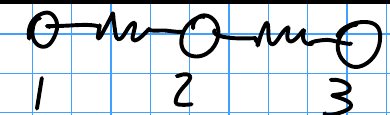
\includegraphics[width=0.35\textwidth]{figures/fig_spring_chain.png}\\[6pt]
  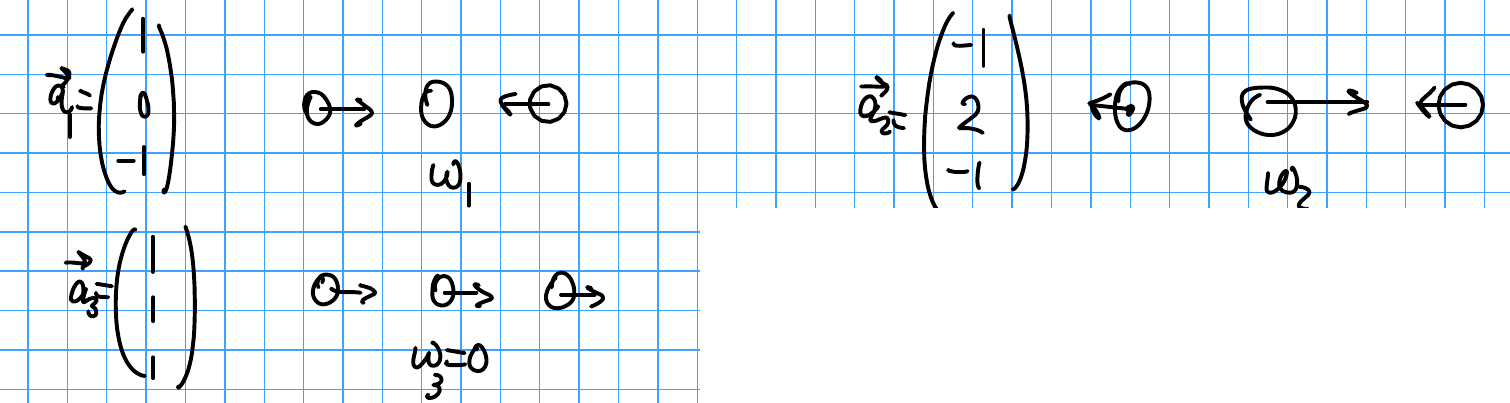
\includegraphics[width=0.95\textwidth]{figures/fig_normal_modes_3mass.png}
  \caption{Three masses $1,2,3$ coupled by two springs, and the three normal modes:
  $\vec a_1 = (1,0,-1)^{\mathsf T}$ with frequency $\omega_1$ (outer masses move
  oppositely, centre mass at rest); $\vec a_2 = (-1,2,-1)^{\mathsf T}$ with
  $\omega_2$; and the uniform translation $\vec a_3 = (1,1,1)^{\mathsf T}$ with
  $\omega_3 = 0$.}
\end{figure}

\begin{equation*}
  \begin{pmatrix}\eta_1\\ \eta_2\\ \eta_3\end{pmatrix}
  = C_1\,\vec a_1 \cos(\omega_1 t + \delta_1)
  + C_2\,\vec a_2 \cos(\omega_2 t + \delta_2)
  + C_3\,\vec a_3 \cos(\omega_3 t + \delta_3)
\end{equation*}

\hrule\vspace{6pt}

\subsection*{Normal coordinate \texorpdfstring{$\zeta$}{zeta}}

\begin{equation*}
  \vec\eta = \Am\,\vec\zeta ,
  \qquad
  \eta_i = \sum_k \zeta_k\, a_{ik} ,
  \qquad
  \zeta_k = C_k \cos(\omega_k t + \delta_k) ,
  \qquad
  \vec\zeta = \Am^{-1}\vec\eta = \Am^{\mathsf T}\,\Tm\,\vec\eta .
\end{equation*}

\begin{align*}
  L &= \frac{1}{2}\sum_{i,j}\bigl(\dot\eta_i\,T_{ij}\,\dot\eta_j - \eta_i\,V_{ij}\,\eta_j\bigr)
     = \frac{1}{2}\Bigl[(\dot{\vec\eta})^{\mathsf T}\,\Tm\,\dot{\vec\eta}
                      - \vec\eta^{\,\mathsf T}\,\Vm\,\vec\eta\Bigr]
     = \frac{1}{2}\Bigl[\dot{\vec\zeta}^{\,\mathsf T}\Am^{\mathsf T}\Tm\Am\dot{\vec\zeta}
                      - \vec\zeta^{\,\mathsf T}\Am^{\mathsf T}\Vm\Am\vec\zeta\Bigr]\\[4pt]
  L &= \frac{1}{2}\Bigl[\dot{\vec\zeta}^{\,\mathsf T}\dot{\vec\zeta}
      - \vec\zeta^{\,\mathsf T}
        \begin{pmatrix}\omega_1^2 & & 0\\ & \ddots & \\ 0 & & \omega_n^2\end{pmatrix}
        \vec\zeta\Bigr]
  \quad\Longrightarrow\quad
  \boxeq{\;L = \frac{1}{2}\sum_{k=1}^{n}\bigl(\dot\zeta_k^2 - \omega_k^2\,\zeta_k^2\bigr)\;}
\end{align*}

\section*{Example: Oscillations of a double pendulum}

\begin{figure}[htbp]
  \centering
  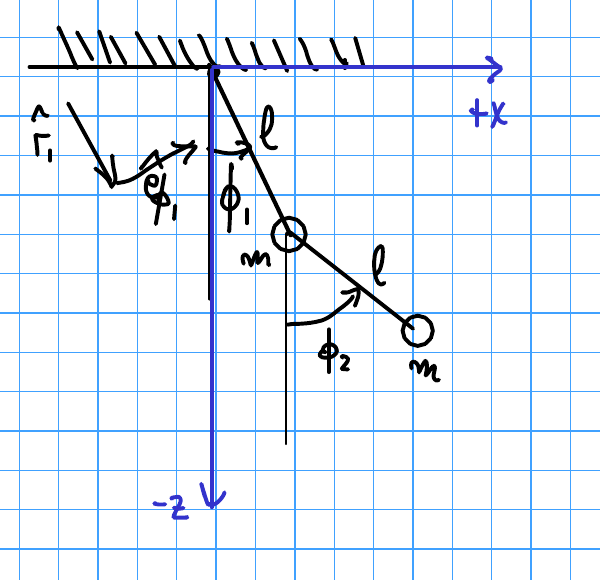
\includegraphics[width=0.42\textwidth]{figures/fig_double_pendulum.png}
  \caption{Two equal masses $m$ on two rods of equal length $l$ hung from a fixed
  ceiling, with angles $\phi_1$, $\phi_2$ measured from the downward vertical, and
  the unit vectors $\unit r_1$, $\unit e_{\phi_1}$. The
  \textcolor{notesblue}{blue} axes fix the sign convention: $+x$ to the right and
  $-z$ \emph{downward}, which is what makes
  $V = -mgl(2\cos\phi_1 + \cos\phi_2)$.}
\end{figure}

\subsection*{Transformation equations}

\begin{align*}
  \vec r_1 &= l\bigl(\sin\phi_1\,\unit x - \cos\phi_1\,\unit z\bigr) = l\,\unit r_1 ,\\
  \vec r_2 &= l\bigl(\sin\phi_1\,\unit x - \cos\phi_1\,\unit z\bigr)
            + l\bigl(\sin\phi_2\,\unit x - \cos\phi_2\,\unit z\bigr)
            = l\bigl(\unit r_1 + \unit r_{21}\bigr) ,\\
  \unit r_1 &= \sin\phi_1\,\unit x - \cos\phi_1\,\unit z ,
  \qquad
  \unit r_{21} = \sin\phi_2\,\unit x - \cos\phi_2\,\unit z .
\end{align*}

\subsection*{Velocities}

\begin{align*}
  \dot{\unit r}_1 &= \dot\phi_1\,\pd{\unit r_1}{\phi_1} ,
    & \pd{\unit r_1}{\phi_1} &= \unit e_{\phi_1} = \cos\phi_1\,\unit x + \sin\phi_1\,\unit z ,\\
  \dot{\unit r}_{21} &= \dot\phi_2\,\pd{\unit r_{21}}{\phi_2} ,
    & \pd{\unit r_{21}}{\phi_2} &= \unit e_{\phi_2} = \cos\phi_2\,\unit x + \sin\phi_2\,\unit z ,
\end{align*}
\begin{align*}
  \dot{\vec r}_1 &= l\,\dot{\unit r}_1 = l\,\dot\phi_1\bigl(\cos\phi_1\,\unit x + \sin\phi_1\,\unit z\bigr),\\
  \dot{\vec r}_2 &= l\bigl(\dot{\unit r}_1 + \dot{\unit r}_{21}\bigr)
    = l\,\dot\phi_1\bigl(\cos\phi_1\,\unit x + \sin\phi_1\,\unit z\bigr)
    + l\,\dot\phi_2\bigl(\cos\phi_2\,\unit x + \sin\phi_2\,\unit z\bigr).
\end{align*}

\begin{align*}
  T &= \frac{m}{2}\Bigl[\bigl(\dot{\vec r}_1\bigr)^2 + \bigl(\dot{\vec r}_2\bigr)^2\Bigr]
     = \frac{m}{2}\Bigl[l^2\dot\phi_1^2
       + l^2\bigl(\dot\phi_1^2 + \dot\phi_2^2
       + 2\dot\phi_1\dot\phi_2\,\unit e_{\phi_1}\cdot\unit e_{\phi_2}\bigr)\Bigr],\\
  \unit e_{\phi_1}\cdot\unit e_{\phi_2}
    &= \cos\phi_1\cos\phi_2 + \sin\phi_1\sin\phi_2 = \cos(\phi_2-\phi_1),\\[4pt]
  T &= \frac{ml^2}{2}\Bigl[2\dot\phi_1^2 + \dot\phi_2^2
       + 2\dot\phi_1\dot\phi_2\cos(\phi_2-\phi_1)\Bigr],\\
  V &= mgz_1 + mgz_2 = -mgl\bigl(2\cos\phi_1 + \cos\phi_2\bigr),\\[4pt]
  L &= T - V = \frac{ml^2}{2}\Bigl[2\dot\phi_1^2 + \dot\phi_2^2
       + 2\dot\phi_1\dot\phi_2\cos(\phi_2-\phi_1)\Bigr]
       + mgl\bigl(2\cos\phi_1 + \cos\phi_2\bigr).
\end{align*}

We know $\phi_1 = \phi_2 = 0$ is stable equilibrium position, but let's
check:\tnote{The first derivative below is as written. For the $V$ above,
$\partial V/\partial\phi_1 = 2mgl\sin\phi_1$; the factor $2$ is absent in the
manuscript. The conclusion --- a stationary point at $\phi_1 = 0$ --- is
unaffected.}
\begin{equation*}
  \pd{V}{\phi_1} = mgl\sin\phi_1 = 0 \ \text{ at } \phi_1 = 0 \ \checkmark
  \qquad\qquad
  \pd{V}{\phi_2} = mgl\sin\phi_2 = 0 \ \text{ at } \phi_2 = 0 \ \checkmark
\end{equation*}
And $V$ is absolute minimum at $\phi_1 = \phi_2 = 0$ $\Rightarrow$ Equil is STABLE.

We thus expand $T$ and $V$ to quadratic order in
$\eta_i = \phi_i - \phi_i^{0} = \phi_i$, since $\phi_i^0 = 0$:
\begin{align*}
  \dot\phi_1\dot\phi_2\cos(\phi_2-\phi_1)
    &= \dot\eta_1\dot\eta_2\cos(\eta_2-\eta_1)
     \simeq \dot\eta_1\dot\eta_2
       \underset{\text{\scriptsize small }\eta_i}
       {\Bigl[1 - \frac{(\eta_2-\eta_1)^2}{2} + \cdots\Bigr]}
     \simeq \dot\eta_1\dot\eta_2 + \rmath{O(\dot\eta^2\eta^2)} ,\\[4pt]
  \cos\phi_i = \cos\eta_i
    &= 1 - \frac{\eta_i^2}{2} + \rmath{\frac{\eta_i^4}{4!}} - \rmath{\cdots}
     \simeq 1 - \frac{\eta_i^2}{2} .
\end{align*}

Thus, to quadratic order in $\eta$ and $\dot\eta$ we get
\begin{align*}
  V &= -mgl\left[3 - \frac{2\eta_1^2}{2} - \frac{\eta_2^2}{2}\right]
   \quad\Longrightarrow\quad
   \Vm = mgl\begin{pmatrix}2 & 0\\ 0 & 1\end{pmatrix},\\[4pt]
  T &= \frac{ml^2}{2}\Bigl[2\dot\eta_1^2 + \dot\eta_2^2 + 2\dot\eta_1\dot\eta_2\Bigr]
   \quad\Longrightarrow\quad
   \Tm = ml^2\begin{pmatrix}2 & 1\\ 1 & 1\end{pmatrix},
\end{align*}
consistent with
$T = \tfrac{1}{2}\bigl(\dot\eta_1 \cdots \dot\eta_n\bigr)\,\Tm\,
     \bigl(\dot\eta_1 \cdots \dot\eta_n\bigr)^{\mathsf T}$.

\medskip
\noindent\textsc{Check.}
\begin{align*}
  \begin{pmatrix}\eta_1 & \eta_2\end{pmatrix}
  \begin{pmatrix}2 & 0\\ 0 & 1\end{pmatrix}
  \begin{pmatrix}\eta_1\\ \eta_2\end{pmatrix}
  &= \begin{pmatrix}\eta_1 & \eta_2\end{pmatrix}
     \begin{pmatrix}2\eta_1\\ \eta_2\end{pmatrix}
   = 2\eta_1^2 + \eta_2^2 \ \checkmark\\
  \begin{pmatrix}\dot\eta_1 & \dot\eta_2\end{pmatrix}
  \begin{pmatrix}2 & 1\\ 1 & 1\end{pmatrix}
  \begin{pmatrix}\dot\eta_1\\ \dot\eta_2\end{pmatrix}
  &= \begin{pmatrix}\dot\eta_1 & \dot\eta_2\end{pmatrix}
     \begin{pmatrix}2\dot\eta_1 + \dot\eta_2\\ \dot\eta_1 + \dot\eta_2\end{pmatrix}
   = 2\dot\eta_1^2 + 2\dot\eta_1\dot\eta_2 + \dot\eta_2^2 \ \checkmark
\end{align*}

\section*{Eigenfrequencies and eigenvectors}

To simplify the algebra, we write
\begin{equation*}
  mgl = ml^2\left(\frac{g}{l}\right),
  \qquad\qquad
  \omega_0^2 \equiv \frac{g}{l} .
\end{equation*}

Eigenvalue equation:
\begin{align*}
  0 = \operatorname{Det}\bigl[\Vm - \omega^2\Tm\bigr]
    &= \operatorname{Det}\left( ml^2
       \begin{bmatrix}
         2\frac{g}{l} - 2\omega^2 & -\omega^2\\[2pt]
         -\omega^2 & \frac{g}{l} - \omega^2
       \end{bmatrix}\right)\\[4pt]
  \iff\quad
  0 &= \bigl(2\omega_0^2 - 2\omega^2\bigr)\bigl(\omega_0^2 - \omega^2\bigr) - \omega^4\\
    &= \rmath{2}\,\omega^4 - 4\omega^2\omega_0^2 + 2\omega_0^4 - \rmath{\omega^4}
     = \omega^4 - 4\omega_0^2\omega^2 + 2\omega_0^4\\[4pt]
  \iff\quad
  0 &= \underset{\text{\scriptsize COMPLETE SQUARES}}{\bigl(\omega^2 - 2\omega_0^2\bigr)^2}
      - \underbrace{\bigl(4\omega_0^4 - 2\omega_0^4\bigr)}_{2\omega_0^4}\\[4pt]
  \iff\quad
  \omega^2 &= 2\omega_0^2 \pm \sqrt{2}\,\omega_0^2 = \bigl(2\pm\sqrt2\bigr)\omega_0^2\\[4pt]
  \iff\quad
  \boxeq{\;\omega =
    \begin{cases}
      \omega_+ = \sqrt{2+\sqrt2}\ \,\omega_0\\[4pt]
      \omega_- = \sqrt{2-\sqrt2}\ \,\omega_0
    \end{cases}\;}
    &\qquad\text{\emph{Eigenfrequencies}}
\end{align*}

Eigenvectors:
\begin{equation*}
  \begin{pmatrix}0\\ 0\end{pmatrix}
  = \begin{pmatrix}
      2\omega_0^2 - 2\omega^2 & -\omega^2\\[2pt]
      -\omega^2 & \omega_0^2 - \omega^2
    \end{pmatrix}
    \begin{pmatrix}a_1\\ a_2\end{pmatrix}
  \iff
  \begin{cases}
    0 = 2\bigl(\omega_0^2-\omega^2\bigr)a_1 - \omega^2 a_2\\[4pt]
    0 = -\omega^2 a_1 + \bigl(\omega_0^2-\omega^2\bigr)a_2
  \end{cases}
\end{equation*}
\begin{equation*}
  \iff
  \begin{cases}
    a_2 = 2\!\left(\dfrac{\omega_0^2}{\omega^2}-1\right) a_1\\[10pt]
    a_1 = \left(\dfrac{\omega_0^2}{\omega^2}-1\right) a_2
  \end{cases}
  \iff
  \begin{cases}
    \dfrac{a_2}{a_1} = 2\!\left(\dfrac{\omega_0^2}{\omega^2}-1\right)\\[12pt]
    \dfrac{a_2}{a_1} = \dfrac{1}{\left(\dfrac{\omega_0^2}{\omega^2}-1\right)}
  \end{cases}
\end{equation*}

\hrule\vspace{4pt}

\noindent\textsc{Side note:} the 2 equations are equivalent:
\begin{align*}
  2\!\left(\frac{\omega_0^2}{\omega^2}-1\right)
    = \frac{1}{\left(\frac{\omega_0^2}{\omega^2}-1\right)}
  &\iff
  1 = 2\!\left(\frac{\omega_0^2}{\omega^2}-1\right)\!\left(\frac{\omega_0^2}{\omega^2}-1\right)\\
  &\iff
  \omega^4 = 2\bigl(\omega_0^2-\omega^2\bigr)\bigl(\omega_0^2-\omega^2\bigr)\\
  &\iff
  0 = 2\bigl(\omega_0^2-\omega^2\bigr)\bigl(\omega_0^2-\omega^2\bigr) - \omega^4
   \iff
  0 = \operatorname{Det}\bigl(\Vm - \omega^2\Tm\bigr) \ \checkmark
\end{align*}

\hrule\vspace{6pt}

So we can take either equation and use it, together with normalization, to get
$\vec a$:
\begin{equation*}
  \text{Propose}\quad
  \vec a = \mathcal{N}
    \begin{pmatrix}1\\[2pt] 2\!\left(\frac{\omega_0^2}{\omega^2}-1\right)\end{pmatrix},
  \qquad \mathcal{N}: \text{normalization constant},
  \qquad x = \frac{\omega_0^2}{\omega^2}.
\end{equation*}

\begin{align*}
  1 = [\vec a\,]^{\mathsf T}\,\Tm\,[\vec a\,]
   &= \mathcal{N}^2\begin{pmatrix}1 & 2(x-1)\end{pmatrix} ml^2
      \begin{pmatrix}2 & 1\\ 1 & 1\end{pmatrix}
      \begin{pmatrix}1\\ 2(x-1)\end{pmatrix}
    = \mathcal{N}^2 ml^2 \begin{pmatrix}1 & 2(x-1)\end{pmatrix}
      \begin{pmatrix}2x\\ 2x-1\end{pmatrix}\\[4pt]
  1 &= \mathcal{N}^2 ml^2\bigl[2x + 2(x-1)(2x-1)\bigr]
     = 2\mathcal{N}^2 ml^2\bigl[2x^2 - 3x + x + 1\bigr]\\
   &= 2\mathcal{N}^2 ml^2\bigl[2x^2 - 2x + 1\bigr]
     = 2\mathcal{N}^2 ml^2\bigl[2(x-1)^2 + 4x - 2 + 1\bigr]\\
   &= 2\mathcal{N}^2 ml^2\Bigl\{\underbrace{\bigl[2(x-1)^2 - 1\bigr]}_{0} + 2x\Bigr\}
     = 4\mathcal{N}^2 ml^2\,\frac{\omega_0^2}{\omega^2}\\[4pt]
  &\Longrightarrow\quad
  \boxeq{\;\mathcal{N}_\pm = \frac{1}{\sqrt{4m}}\,\frac{\omega_\pm}{l\,\omega_0}
    = \left(\frac{2\pm\sqrt2}{4ml^2}\right)^{1/2}\;}
\end{align*}

\noindent Supporting algebra:\tnote{In the third line above, the term $-2x$ is
absent from the bracket $[2(x-1)^2 + 4x - 2 + 1]$; transcribed as written. The
lecturer's own side computation immediately below carries it:
$2x^2-2x+1 = 2[(x-1)^2+2x-1] - 2x + 1 = [2(x-1)^2-1]+2x$, which is what the next
equality uses.}
\begin{gather*}
  (x-1)^2 = x^2 - 2x + 1 ,
  \qquad x^2 = (x-1)^2 + 2x - 1 ,\\
  2x^2 - 2x + 1 = 2\bigl[(x-1)^2 + 2x - 1\bigr] - 2x + 1 = \bigl[2(x-1)^2 - 1\bigr] + 2x ,\\[4pt]
  \omega^4\bigl[2(x-1)^2 - 1\bigr]
    = \bigl[2\bigl(x\omega^2 - \omega^2\bigr)^2 - \omega^4\bigr]
    = \bigl[2\bigl(\omega_0^2 - \omega^2\bigr)^2 - \omega^4\bigr] = 0 .
\end{gather*}

\begin{gather*}
  \frac{\omega_0^2}{\omega_\pm^2} = \frac{1}{2\pm\sqrt2}
    = \frac{2\mp\sqrt2}{4-2} = 1 \mp \frac{1}{\sqrt2} ,
  \qquad\qquad
  2\left[\frac{\omega_0^2}{\omega_\pm^2} - 1\right] = \mp\sqrt2 ,\\[6pt]
  \boxeq{\;\vec a_\pm = \left(\frac{2\pm\sqrt2}{4ml^2}\right)^{1/2}
    \begin{pmatrix}1\\ \mp\sqrt2\end{pmatrix}\;}
  \qquad\Longleftrightarrow\qquad
  \boxeq{\;\omega_\pm = \left[\bigl(2\pm\sqrt2\bigr)\frac{g}{l}\right]^{1/2}\;}
\end{gather*}

\medskip
\noindent Modal matrix:
\begin{equation*}
  \boxeq{\;
    \Am = \bigl(\vec a_+\ \ \vec a_-\bigr)
    = \bigl(4ml^2\bigr)^{-1/2}\begin{pmatrix}a & b\\ c & d\end{pmatrix}\;}
\end{equation*}
\begin{align*}
  a &\equiv \bigl(2+\sqrt2\bigr)^{1/2} = -c/\sqrt2 ,
    & c &= -\sqrt2\,a = -\sqrt2\bigl(2+\sqrt2\bigr)^{1/2} ,\\
  b &\equiv \bigl(2-\sqrt2\bigr)^{1/2} = d/\sqrt2 ,
    & d &= +\sqrt2\,b = +\sqrt2\bigl(2-\sqrt2\bigr)^{1/2} .
\end{align*}

\section*{Graphical representation}

\begin{figure}[htbp]
  \centering
  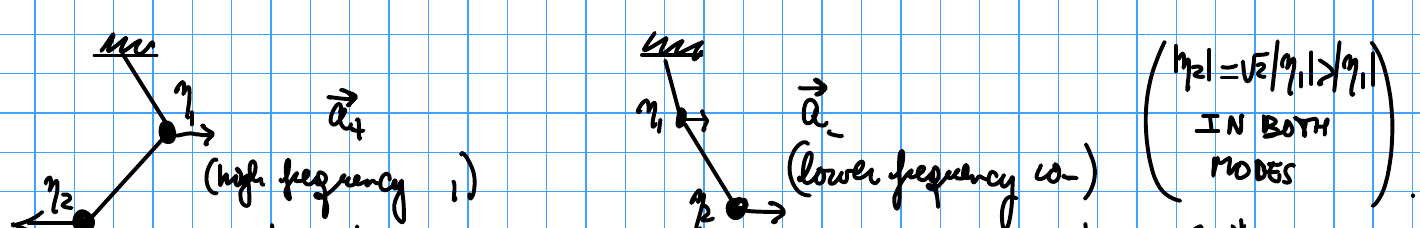
\includegraphics[width=\textwidth]{figures/fig_modes_pm.png}
  \caption{The two normal modes of the double pendulum. Left: $\vec a_+$, the
  high-frequency mode $\omega_+$, in which the two bobs move in opposite senses.
  Right: $\vec a_-$, the lower-frequency mode $\omega_-$, in which they move
  together. In both modes $|\eta_2| = \sqrt2\,|\eta_1| > |\eta_1|$.}
\end{figure}

\subsection*{Normal coordinates}

\begin{align*}
  \vec\zeta &= \Am^{\mathsf T}\,\Tm\,\vec\eta
    = \Am^{\mathsf T}\, ml^2 \begin{pmatrix}2 & 1\\ 1 & 1\end{pmatrix}
      \begin{pmatrix}\eta_1\\ \eta_2\end{pmatrix}\\[4pt]
  \vec\zeta &= \bigl(4ml^2\bigr)^{-1/2}\begin{pmatrix}a & c\\ b & d\end{pmatrix}
     ml^2 \begin{pmatrix}2\eta_1 + \eta_2\\ \eta_1 + \eta_2\end{pmatrix}
   = \left(\frac{ml^2}{4}\right)^{1/2}
     \begin{pmatrix}(2a+c)\eta_1 + (a+c)\eta_2\\[4pt] (2b+d)\eta_1 + (b+d)\eta_2\end{pmatrix}
\end{align*}

\noindent with
\begin{align*}
  2a+c &= \bigl(2-\sqrt2\bigr) a
        = \sqrt2\,\bigl(\sqrt2-1\bigr)^{1/2}\bigl(\sqrt2-1\bigr)^{1/2}\bigl(2+\sqrt2\bigr)^{1/2}
        = \sqrt2\;2^{1/4}\bigl(\sqrt2-1\bigr)^{1/2},\\
  a+c  &= \bigl(1-\sqrt2\bigr) a
        = -\bigl(\sqrt2-1\bigr)^{1/2}\bigl(\sqrt2-1\bigr)^{1/2}\bigl(2+\sqrt2\bigr)^{1/2}
        = -2^{1/4}\bigl(\sqrt2-1\bigr)^{1/2},\\
  2b+d &= \bigl(2+\sqrt2\bigr) b
        = \sqrt2\,\bigl(\sqrt2+1\bigr)^{1/2}\bigl(\sqrt2+1\bigr)^{1/2}\bigl(2-\sqrt2\bigr)^{1/2}
        = \sqrt2\;2^{1/4}\bigl(\sqrt2+1\bigr)^{1/2},\\
  b+d  &= \bigl(1+\sqrt2\bigr) b
        = \bigl(\sqrt2+1\bigr)^{1/2}\bigl(\sqrt2+1\bigr)^{1/2}\bigl(2-\sqrt2\bigr)^{1/2}
        = 2^{1/4}\bigl(\sqrt2+1\bigr)^{1/2},
\end{align*}
where
\begin{equation*}
  \bigl(\sqrt2\mp1\bigr)^{1/2}\bigl(2\pm\sqrt2\bigr)^{1/2}
    = 2^{1/4}\bigl(\sqrt2\mp1\bigr)^{1/2}\bigl(\sqrt2\pm1\bigr)^{1/2} = 2^{1/4},
\end{equation*}
\begin{equation*}
  \left(\frac{ml^2}{4}\right)^{1/2} = m^{1/2}\,\frac{l}{2},
  \qquad\qquad
  \frac{1}{2}\,2^{1/4}\bigl(\sqrt2\mp1\bigr)^{1/2}
    = \left(\frac{\sqrt2\mp1}{2\sqrt2}\right)^{1/2}.
\end{equation*}

\begin{gather*}
  \boxeq{\;
  \begin{aligned}
    \zeta_+(t) &= m^{1/2} l \left(\frac{\sqrt2-1}{2\sqrt2}\right)^{1/2}
                  \bigl[\sqrt2\,\eta_1(t) - \eta_2(t)\bigr]\\[4pt]
    \zeta_-(t) &= m^{1/2} l \left(\frac{\sqrt2+1}{2\sqrt2}\right)^{1/2}
                  \bigl[\sqrt2\,\eta_1(t) + \eta_2(t)\bigr]
  \end{aligned}\;}\\[10pt]
  \boxeq{\;
  \begin{aligned}
    \dot\zeta_+(t) &= m^{1/2} l \left(\frac{\sqrt2-1}{2\sqrt2}\right)^{1/2}
                  \bigl[\sqrt2\,\dot\eta_1(t) - \dot\eta_2(t)\bigr]\\[4pt]
    \dot\zeta_-(t) &= m^{1/2} l \left(\frac{\sqrt2+1}{2\sqrt2}\right)^{1/2}
                  \bigl[\sqrt2\,\dot\eta_1(t) + \dot\eta_2(t)\bigr]
  \end{aligned}\;}
\end{gather*}

But we know also that:
\begin{gather*}
  \boxeq{\;
  \begin{aligned}
    \zeta_+(t) &= f_+\cos(\omega_+ t + \delta_+)\\[4pt]
    \zeta_-(t) &= f_-\cos(\omega_- t + \delta_-)
  \end{aligned}\;}
  \qquad
  \boxeq{\;
  \begin{aligned}
    \dot\zeta_+(t) &= -f_+\,\omega_+\sin(\omega_+ t + \delta_+)\\[4pt]
    \dot\zeta_-(t) &= -f_-\,\omega_-\sin(\omega_- t + \delta_-)
  \end{aligned}\;}
\end{gather*}

\subsection*{Lagrangian in terms of the normal coordinates}

\begin{align*}
  L &= \frac{1}{2}\sum_\alpha\bigl(\dot\zeta_\alpha^2 - \omega_\alpha^2\zeta_\alpha^2\bigr)
     = \frac{1}{2}\Bigl[\bigl(\dot\zeta_+^2 - \omega_+^2\zeta_+^2\bigr)
                      + \bigl(\dot\zeta_-^2 - \omega_-^2\zeta_-^2\bigr)\Bigr]\\[4pt]
  L &= \frac{1}{2}\left[\left(\dot\zeta_+^2 - \Bigl[\bigl(2+\sqrt2\bigr)\frac{g}{l}\Bigr]\zeta_+^2\right)
      + \left(\dot\zeta_-^2 - \Bigl[\bigl(2-\sqrt2\bigr)\frac{g}{l}\Bigr]\zeta_-^2\right)\right]
\end{align*}

\section*{Solution for a given initial condition}

Assume initial condition is that at $t=0$:
\begin{equation*}
  \phi_1 = \phi_2 = 0,
  \qquad\qquad
  \dot\phi_1 = -\dot\phi_2 = \nu > 0 .
\end{equation*}

\noindent\underline{Get $\phi_1(t)$, $\phi_2(t)$.} Then
\begin{align*}
  f_+\cos(\delta_+) &= \zeta_+(0) = 0
    \quad\Longrightarrow\quad \delta_+ = \pm\frac{\pi}{2},\ \pm\frac{3}{2}\pi,\ \dots\\
  f_-\cos(\delta_-) &= \zeta_-(0) = 0
    \quad\Longrightarrow\quad \delta_- = \pm\frac{\pi}{2},\ \pm\frac{3}{2}\pi,\ \dots
\end{align*}
\begin{align*}
  -f_+\omega_+\sin(\delta_+) &= \dot\zeta_+(0)
    = m^{1/2} l \left(\frac{\sqrt2-1}{2\sqrt2}\right)^{1/2}\bigl[\sqrt2\,\nu - (-\nu)\bigr]
    = \sqrt{2+\sqrt2}\;\frac{m^{1/2} l\,\nu}{2},\\
  -f_-\omega_-\sin(\delta_-) &= \dot\zeta_-(0)
    = m^{1/2} l \left(\frac{\sqrt2+1}{2\sqrt2}\right)^{1/2}\bigl[\sqrt2\,\nu + (-\nu)\bigr]
    = \sqrt{2-\sqrt2}\;\frac{m^{1/2} l\,\nu}{2},
\end{align*}
using
\begin{equation*}
  m^{1/2} l \left(\frac{\sqrt2\mp1}{2\sqrt2}\right)^{1/2}\bigl(\sqrt2\pm1\bigr)\nu
  = \left(\frac{\sqrt2\pm1}{2\sqrt2}\right)^{1/2} m^{1/2} l\,\nu
  = \sqrt{2\pm\sqrt2}\;\frac{m^{1/2} l\,\nu}{2}.
\end{equation*}

Choose $\delta_+ = \delta_- = -\dfrac{\pi}{2}$:
\begin{equation*}
  \Longrightarrow\quad
  f_\pm\,\sqrt{2\pm\sqrt2}\,\sqrt{\frac{g}{l}}
    = \sqrt{2\pm\sqrt2}\;\frac{m^{1/2} l\,\nu}{2}
  \quad\Longrightarrow\quad
  \boxeq{\;f_\pm = \frac{\nu}{2}\left[\frac{ml^3}{g}\right]^{1/2}\;}
\end{equation*}
\begin{equation*}
  \cos\!\left(\omega t - \frac{\pi}{2}\right)
   = \cos\omega t\;\overset{0}{\rmath{\cos\frac{\pi}{2}}}
   + \sin\omega t\;\underset{1}{\boxed{\sin\frac{\pi}{2}}}
   = \sin\omega t
\end{equation*}

\begin{equation*}
  \zeta_\pm(t) = f_\pm\cos\!\left(\omega_\pm t - \frac{\pi}{2}\right) = f_\pm\sin(\omega_\pm t)
\end{equation*}
\begin{equation*}
  \boxeq{\;\zeta_\pm(t) = \frac{\nu}{2}\left[\frac{ml^3}{g}\right]^{1/2}
    \sin\!\left(\left[\bigl(2\pm\sqrt2\bigr)\frac{g}{l}\right]^{1/2} t\right)\;}
\end{equation*}

\noindent with
\begin{align*}
  a &\equiv \bigl(2+\sqrt2\bigr)^{1/2} = 2^{1/4}\bigl(\sqrt2+1\bigr)^{1/2},
    & c &= -\sqrt2\,a,
    & f_+ a &= \frac{\nu}{2}\left[\frac{ml^3}{g}\right]^{1/2}\bigl(2+\sqrt2\bigr)^{1/2},\\
  b &\equiv \bigl(2-\sqrt2\bigr)^{1/2} = 2^{1/4}\bigl(\sqrt2-1\bigr)^{1/2},
    & d &= +\sqrt2\,b,
    & f_- b &= \frac{\nu}{2}\left[\frac{ml^3}{g}\right]^{1/2}\bigl(2-\sqrt2\bigr)^{1/2},
\end{align*}
\begin{equation*}
  \bigl(4ml^2\bigr)^{-1/2}\,\frac{\nu}{2}\left(\frac{ml^3}{g}\right)^{1/2}
  = \frac{\nu}{4\sqrt{\frac{g}{l}}} .
\end{equation*}

\subsection*{In terms of the original coordinates}

\begin{equation*}
  \vec\eta(t) = \Am\,\vec\zeta(t)
  = \bigl(4ml^2\bigr)^{-1/2}\begin{pmatrix}a & b\\ c & d\end{pmatrix}
    \begin{pmatrix}\zeta_+(t)\\ \zeta_-(t)\end{pmatrix}
  = \bigl(4ml^2\bigr)^{-1/2}
    \begin{pmatrix}a\,\zeta_+(t) + b\,\zeta_-(t)\\[2pt] c\,\zeta_+(t) + d\,\zeta_-(t)\end{pmatrix}
\end{equation*}

\begin{equation*}
  \boxeq{\;
  \begin{aligned}
    \phi_1(t) = \eta_1(t)
      &= \frac{\nu}{4\sqrt{\frac{g}{l}}}
         \Bigl\{\bigl(2+\sqrt2\bigr)^{1/2}
           \sin\!\left(\Bigl[\bigl(2+\sqrt2\bigr)\tfrac{g}{l}\Bigr]^{1/2} t\right)\\
      &\hspace{4.2em}+ \bigl(2-\sqrt2\bigr)^{1/2}
           \sin\!\left(\Bigl[\bigl(2-\sqrt2\bigr)\tfrac{g}{l}\Bigr]^{1/2} t\right)\Bigr\}\\[8pt]
    \phi_2(t) = \eta_2(t)
      &= \frac{\sqrt2\,\nu}{4\sqrt{\frac{g}{l}}}
         \Bigl\{-\bigl(2+\sqrt2\bigr)^{1/2}
           \sin\!\left(\Bigl[\bigl(2+\sqrt2\bigr)\tfrac{g}{l}\Bigr]^{1/2} t\right)\\
      &\hspace{4.2em}+ \bigl(2-\sqrt2\bigr)^{1/2}
           \sin\!\left(\Bigl[\bigl(2-\sqrt2\bigr)\tfrac{g}{l}\Bigr]^{1/2} t\right)\Bigr\}
  \end{aligned}\;}
\end{equation*}

\typednote{Check initial condition: At t=0, all sin(\dots) terms are zero, so we
have:}
\begin{equation*}
  \phi_1 = \phi_2 = 0 \quad\checkmark
\end{equation*}

\begin{equation*}
  \boxeq{\;
  \begin{aligned}
    \dot\phi_1(t) = \dot\eta_1(t)
      &= \frac{\nu}{4}
         \Bigl\{\bigl(2+\sqrt2\bigr)
           \cos\!\left(\Bigl[\bigl(2+\sqrt2\bigr)\tfrac{g}{l}\Bigr]^{1/2} t\right)\\
      &\hspace{2.6em}+ \bigl(2-\sqrt2\bigr)
           \cos\!\left(\Bigl[\bigl(2-\sqrt2\bigr)\tfrac{g}{l}\Bigr]^{1/2} t\right)\Bigr\}\\[8pt]
    \dot\phi_2(t) = \dot\eta_2(t)
      &= \frac{\sqrt2\,\nu}{4}
         \Bigl\{-\bigl(2+\sqrt2\bigr)
           \cos\!\left(\Bigl[\bigl(2+\sqrt2\bigr)\tfrac{g}{l}\Bigr]^{1/2} t\right)\\
      &\hspace{2.6em}+ \bigl(2-\sqrt2\bigr)
           \cos\!\left(\Bigl[\bigl(2-\sqrt2\bigr)\tfrac{g}{l}\Bigr]^{1/2} t\right)\Bigr\}
  \end{aligned}\;}
\end{equation*}

\typednote{Check initial condition: At t=0, all cos(\dots) terms are 1, so we have:}
\begin{align*}
  \dot\phi_1 &= \frac{\nu}{4}\Bigl\{\bigl(2+\sqrt2\bigr) + \bigl(2-\sqrt2\bigr)\Bigr\}
    = \nu \quad\checkmark\\
  \dot\phi_2 &= \frac{\sqrt2\,\nu}{4}\Bigl\{-\bigl(2+\sqrt2\bigr) + \bigl(2-\sqrt2\bigr)\Bigr\}
    = -\nu \quad\checkmark
\end{align*}

\section*{Comparison with quantum mechanics}

\begin{figure}[htbp]
  \centering
  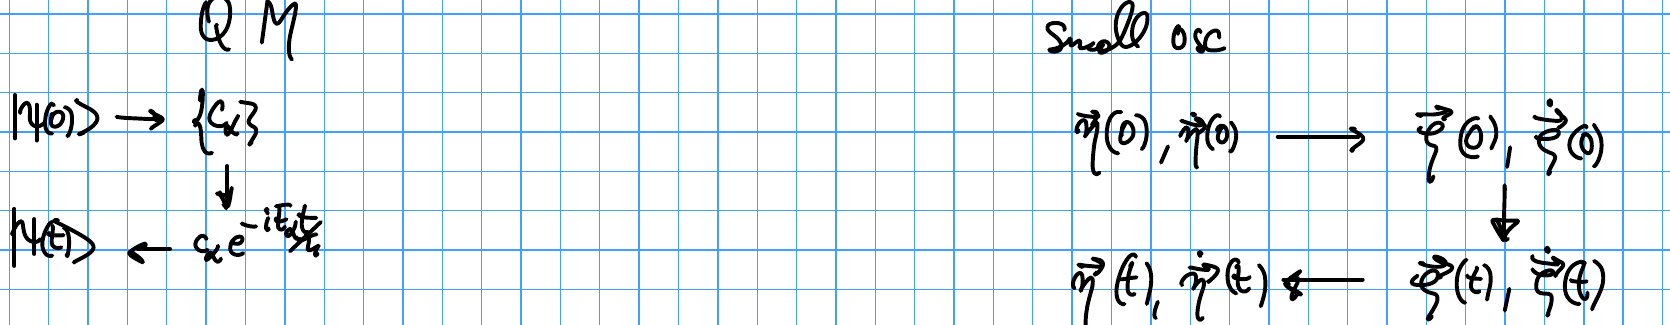
\includegraphics[width=\textwidth]{figures/fig_qm_comparison.png}
  \caption{The two schemes side by side. Left (QM): the initial state
  $\ket{\psi(0)}$ is resolved into the coefficients $\{c_\alpha\}$, each is
  propagated by $c_\alpha e^{-iE_\alpha t/\hbar}$, and the result is reassembled
  into $\ket{\psi(t)}$. Right (small osc): $\vec\eta(0),\dot{\vec\eta}(0)$ are
  mapped to $\vec\zeta(0),\dot{\vec\zeta}(0)$, propagated as
  $\vec\zeta(t),\dot{\vec\zeta}(t)$, and mapped back.}
\end{figure}

\begin{center}
\begin{minipage}[t]{0.46\textwidth}
\begin{center}\textbf{QM}\end{center}
\begin{gather*}
  \ket{\psi(0)} = \sum_\alpha c_\alpha \ket{\varphi_\alpha},
  \qquad c_\alpha = \braket{\varphi_\alpha}{\psi(0)}\\[4pt]
  \ket{\psi(t)} = \sum_\alpha c_\alpha\, e^{-iE_\alpha t/\hbar}\,\ket{\varphi_\alpha}
\end{gather*}
\end{minipage}\hfill
\begin{minipage}[t]{0.46\textwidth}
\begin{center}\textbf{Small osc}\end{center}
\begin{gather*}
  \vec\eta(t) = \Am\,\vec\zeta(t)\\[4pt]
  \vec\zeta(t) = \Am^{\mathsf T}\,\Tm\,\vec\eta(t)
\end{gather*}
\end{minipage}
\end{center}

\end{document}
